\documentclass[dvipdfmx,twocolumn,10.5pt]{jsarticle}
\usepackage[top=30truemm,bottom=27truemm,left=18truemm,right=18truemm,headsep=10truemm]{geometry}
\usepackage{graphicx}
\usepackage{color}
\usepackage{latexsym}
\usepackage{amsmath}
\usepackage[psamsfonts]{amssymb}
\usepackage{txfonts}
\usepackage{url}
\usepackage{colortbl,array,xcolor}
\usepackage{here}
\usepackage{multirow}
\usepackage{comment}
\usepackage[deluxe]{otf}
\usepackage{bm}


\title{越境ECのための商品レビューに基づく評価予測}
\author{大塚 悠貴}
\date{\today}

\begin{document}

\begin{comment}
% コメント
\end{comment}


\twocolumn[
\maketitle
%abstract
% 端的に「結局のところこの論文では何をやったか」=>この論文では~を提案する (まだ書いてない)]
本研究では,越境ECのようなレビューがまだ存在しないドメインにおける商品のレビューのスコアを予測するタスクとその手法を提案する.レビュー文からそのレビュースコアの予測するタスクや感情を分類するタスクと似たタスクであるが,従来の研究ではレビューの文とレビューのスコアが同一のユーザグループによって与えられていることが前提となっている.しかし,越境ECにおいて新たに出品したいその商品のレビューはそのドメインにおいてはまだ存在せず,別のドメインのレビューを参考にせざるを得ない.このような場合には,従来のスコア予測のような手法では,異なる文化背景を捉えることができず,うまく予測できないと考えられる.我々は,マルチタスク学習を用いて,あるドメインのレビュー文から,対象となるドメインにおけるレビューの文とスコアを同時に学習することによって,レビュー文の変化,すなわち文化的な背景を考慮して,スコアを予測することを可能とした.実験では,Amazonのアメリカとイギリスにおける公開データセットを用いて,マルチタスク学習を用いた場合と用いない場合を比較し,マルチタスク学習がこのようなタスクにおいて有効であること明らかにした.
]
%affiliation
\footnote[0]{所属: 社会情報モデル講座・分散情報システム分野\\(指導教員: 吉川 正俊)}

\section{はじめに}
% 1. 研究内容の重要性に直結するような社会的背景
% 越境ECが盛り上がってる && レビューを元に購買意思決定をすることが多くなっている => 越境ECにおけるレビューの予測が重要だが,なかなか難しい
近年,インターネットやスマートフォンの普及に伴い,Amazonや天猫商城などの越境ECと呼ばれる「国境を超えて行われるECサイトの取引」の市場規模が年々拡大している.経済産業省の報告によると,世界の越境ECの市場規模は毎年,対前年$20\%$以上で成長しており,2020年には市場規模が109兆円になると見込まれている\footnote{\url{https://www.meti.go.jp/policy/it_policy/statistics/outlook/H30_hokokusho_new.pdf}}.越境ECでは商圏が限定されず,かつ現地に出店する場合と比べても安く,早く開業することができるため,大企業,中小企ともに参入が続いている.このようにメリットも多い越境ECだが,デメリットもある.自国(以下では国$S$と呼ぶ)で売れているものが新たに販売する対象となる国(以下では国$T$と呼ぶ\footnote{ここでは$S$と$T$は国として表現しているが,厳密には異なるユーザグループをもつドメインのことである})でも同様に売れるとは限らないため,国$T$に在庫を確保したにも関わらず,売れずに損をするというリスクが存在している.さらに,近年はレビューを参考に商品購買の意思決定が行われることが多くなり,どのようなレビューを獲得するかの重要度が増してきている.しかし,国$S$で売っている商品のレビュー文とそのスコアはわかるが,その商品を国$T$で新たに売る際には,当然その商品のレビューが国$T$にはまだ存在しないため,国$T$でどのようなレビューを獲得するかがわからないという問題がある.実際に44\%もの商品がアメリカでの評価よりもイギリスでの評価は低いものとなっている.事前にどのように国$T$でのレビューが国$S$のレビューから変化するのかを予測することが,越境ECにおける出品戦略では重要となる.

% 2. 現状とその問題 どのような研究が行われているか,研究の引用,既存の手法の問題点
% 現状そのような研究は行われていない 既存手法はすでに存在するレビューを感情分析したり,スコアを予測したり
% 今回の問題は予測したい対象にレビューが存在せず,既存手法やろうと思うと,対象国のレビューを考慮しないものになる
% ある商品のレビューから,その商品の評価を予測するに際し,最もよく用いられる手法に感情分析がある.レビューの感情分析は,レビューからユーザの考えを把握すると 同時にユーザが抱く感情を分析することを目的とする技術である.
% ある商品について,レビューからスコアを予測するものや,カテゴリを考慮しない感情分析を行うもの[2]はあるが,越境ECのようなまだレビューが存在しない商品のスコアを予測するという研究は行われていない.国が異なる場合,文化的な違いから,商品に対して受ける印象が大きく異なる場合があるため,別の国レビューを単純につかうということはできない.
従来行われてきた感情分析やスコア予測の多くでは,学習用レビュー文と予測するスコアは同一のユーザーグループによって与えられたものを用いて学習を行っている.しかし,越境ECにおいて新たに商品を出品を検討する際には,レビューのスコアを予測したい商品にはまだレビューは存在しないため,従来の手法の問題設定とは異なることがわかる.このように越境ECを想定した,まだ商品が売られていない地域において,どのようなレビューが得られるかを考察した研究は行われていない.例えば,アメリカではカード決済が主流で,現金を持ち歩区ことが少ないため,長財布より二つ折りの財布が「コンパクトである」と人気であるのに対して,日本ではそういった商品は「思っていたより小さかった」「お札の端が見えるくらいギリギリの大きさ」といったレビューを獲得することがある.実際にAmazon.co.jpでは財布売れ筋ランキング上位10件中6件が長財布(2019年8月31日16:00時点)であるのに対して,Amazon.comでは,財布の売れ筋ランキング上位100件までみても長財布は一件も存在しない(2019年8月31日16:00時点).従来手法において,国$S$の商品レビュー文を入力として,国$T$の商品のレビューのスコアを出力とすると,どのようにその商品のレビューが変わったかという情報が考慮されず,新しい商品に対して適切にスコアの変化を予測できない場合があると考えられる.上記の例では「コンパクト」や「小さい」といった単語がアメリカでは肯定的に,日本では否定的に捉えられたが,収納ケースのような場合では,「小さい」という単語がアメリカでは否定的,日本では肯定的に捉えられる場合がある.つまり,ある単語は国と商品の組み合わせによっては肯定的な単語にも否定的な単語にもなりうる.これはレビューのコンテキストから,その単語がどのようにお互いの国で使われたのかを認識しなければ,一つ目の例を学習した際に,単純に「コンパクト」という単語があると,アメリカでは肯定的だが,日本では否定的と学習してしまう可能性があることを示している.


% TODO: - パワポで作成→illustratorにコピーしてepsで出力 or illustratorで作成しepsで出力
\begin{figure}[tb]
	\centering
	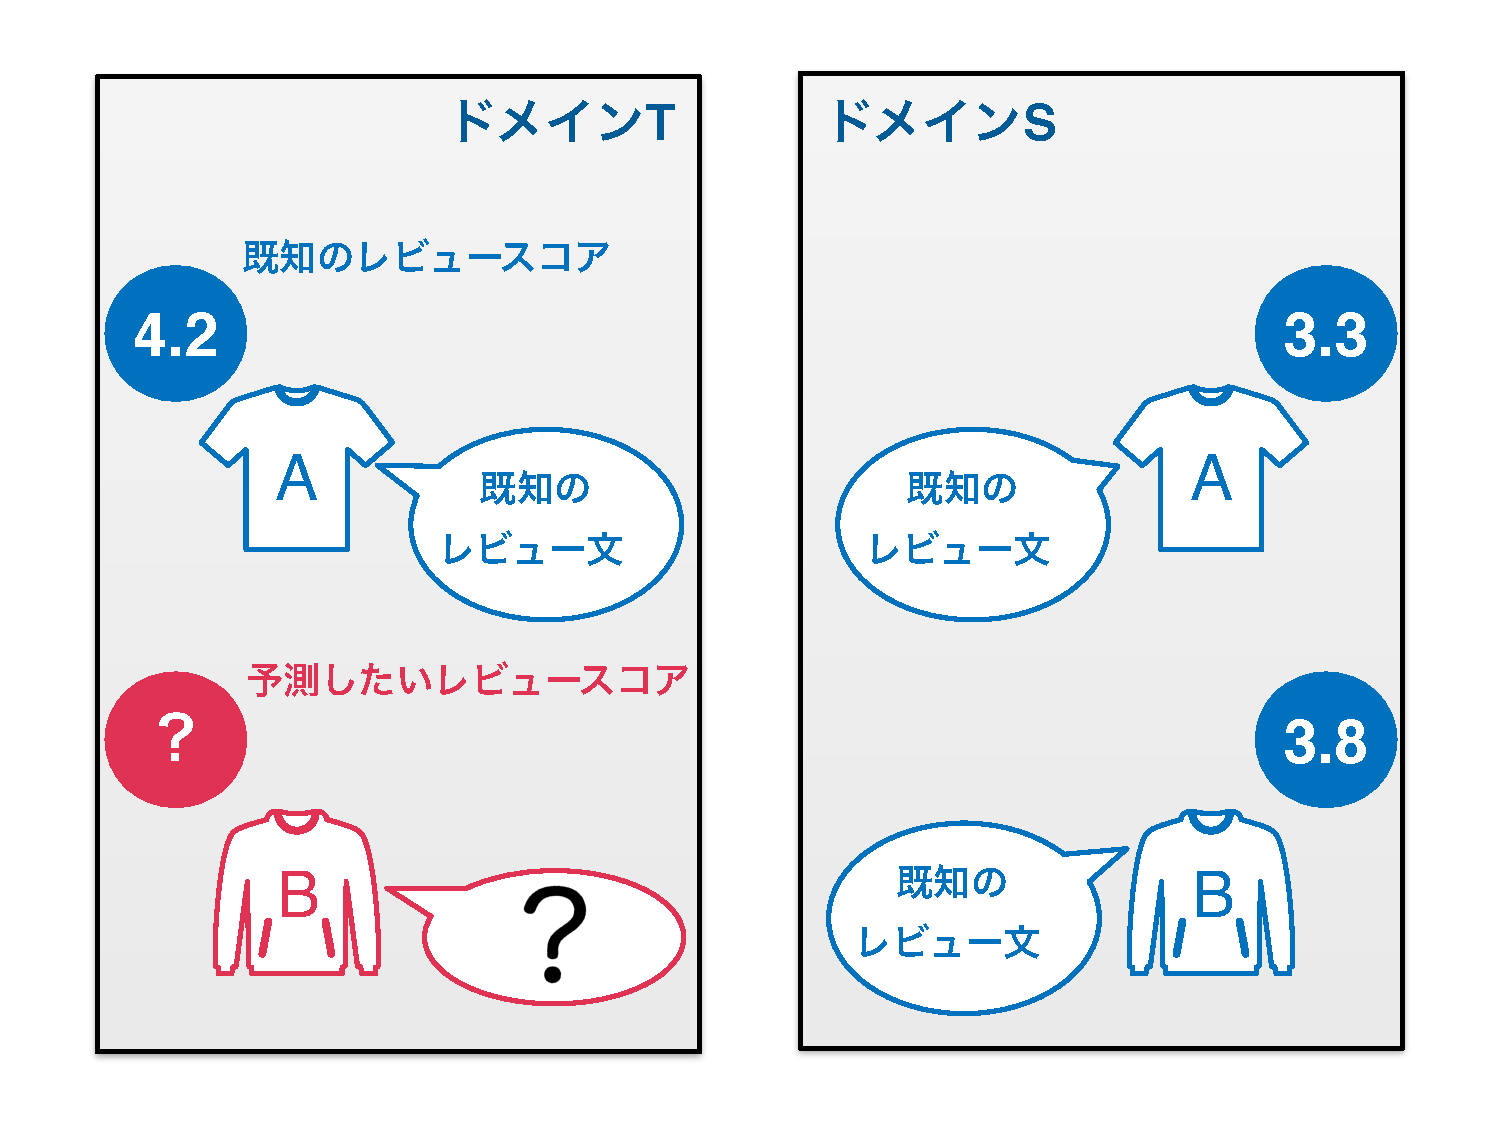
\includegraphics[width=7cm]{images/problem_setting.pdf} 
	\caption{問題設定}
	\label{problem_setting}
\end{figure}

% 3. 提案 (短くてもいい)
% 第1,第2パラグラフで提案内容の重要性の補強をしっかりと行えているか??
% 提案内容の重要性 = 越境ECでレビューを予測する
% シンプルに書くと,レビューが存在しない商品もスコアを予測します
% 第2パラグラフで指摘した問題がそれによって解けるこ とがわかる程度の内容
% ここで問題設定の図を導入してよい
図\ref{problem_setting}は本論文の問題設定である.
我々は国$T$においてまだレビュー文が存在しない商品のスコアを予測するタスクについて,国$T$と国$S$どちらの国でも売られていて,レビュー文とレビュースコアが存在している商品の国$S$におけるレビューの文と国$T$におけるレビュー文から,国$T$のレビュースコアを出力として学習し,国$S$のレビューの文から国$T$におけるレビュー文が存在していない商品のレビュースコアを予測するモデルについての研究を行っている.
国$S$でも国$T$でもすでに販売されている商品のレビューの文を用いることによって,文化的な違いから生じる商品への感情の変化を考慮する.本論文では,越境ECにおいて出品したい商品を,国$T$で販売した際に,国$S$よりも良い評価を得られるかどうかを予測する2値分類問題と,レビューのスコアがどの程度変化するかを予測する回帰問題を考える.

% 4. 提案の実現方法 アイデアを重視 => multitask learning
% 特定のモデル(ニューラルネットワーク,教師ありの機械学習,とかそういう情報も入れてもいい)で取り組んでいる
% レビューの文って明確に言ったほうがいい attention cnn rnn使ってます
% 上記をした上で,multitask learningを使ってる
% 共通に売られている商品が少ないから訓練データが少なって=>
% - 訓練データが少ない時にメリットになる
% 相手のレビューを予測するっていうタスクは別のドメインの点数を予測するっていうのはかなり似たタスク
% レビューの文からスコアを予測するのは精度がよかった
% multitask learningで同時に予測するタスクとしてはよい
本論文では,教師ありの機械学習にニューラルネットを用いて,取り組んでいる.具体的には,入力となるレビューの文に対して,RNN, Attetionを用いている.さらに,本論文では国$S$,国$T$共通で販売されていて,かつ,十分なレビュー数が存在する商品で学習するため,訓練データが少ないという問題がある.実際に,本研究で用いたデータセットにおいて,アメリカの商品$86,813$商品に対し,イギリスでも同様に売られていた商品は$29,426$件,日本では$21,511$件であった.
この問題に対し,本論文ではマルチタスク学習を用いて取り組んでいる.$S$国のレビューの文から$S$国のレビューのスコアを予測する予備実験において,精度が90\%以上あったことから,レビューの文とレビューのスコアは強く関連することがわかる.すなわち,$S$国のレビュー文から$T$国のレビューの文を予測するタスクと,$T$国のスコアを予測するタスクは非常に似たタスクであることがわかる.よって,このように関連する二つのタスクと少ない訓練データを扱う本問題において,Multitask Learningを用いることは適切であると考えられる.

% 5. 実験内容 (設定も含める)
%  - 今回使ったデータの話 => 英米,日英,日米でデータにどんな差があったか,
%  - 今回やったタスクの実験 => multitask(提案手法)はこの問題において効果的であった???
実験では,Amazonが公開する各国で販売されている商品のレビューの文とスコア[3]のうち,アメリカとイギリスで共通して販売されている商品のデータセットを用いた.表\ref{num_of_data}は,アメリカとイギリスで共通して販売されている商品数と各国におけるレビュー数である.
% アメリカとイギリスのスコアの分布は図hogeとhogeに示されるように,近しい分布を持っていることがわかる.
また,アメリカとイギリス両国において,レビューを10以上獲得した商品のスコアの差の分布を示したものが,図\ref{score_diff}である.
% スコアの差が0.4以上存在するものは全体の16.4\%であり,
平均で,0.24のスコアの差が存在することがわかる.,$T$国で販売した際に,$S$国よりも良い評価を得られるかどうかを予測する2値分類問題においては,SVMが54\%の精度,Attentionモデルが56\%の精度であったのに対し,Multitask Learningを用いた手法では58\%の精度であった.また,レビューのスコアがどの程度変化するかを予測する回帰問題においては,平均二乗誤差がSVCは0.26であったのに対し,Multitask Learningを用いた手法は0.1であった.本論文の問題設定において,Multitask Learningを用いることは,一定効果的であったと言える.

% 6. 本論文の貢献
% - 新しいタスクの提案
% - この問題におけるmultitask learningによる手法を提案した => 実験で有効であることを示した
% - 同一商品であっても,国によってレビューが異なる場合があるということを示した
本論文における貢献は,これまで研究されてこなかった越境ECにおける商品レビューに基づくスコア予測のタスクを提案し,この問題においてマルチタスク学習が有効であることを示したことである.

% 7. 本論文の構成
本論文の構成は次の通りである.第2節で感情分析とマルチタスク学習に関わる研究について述べた後,第3節で本論文で提案する越境ECにおける商品レビューに基づく評価予測について説明する.第4節では越境ECにおける商品レビューに基づく評価予測の実現に向けて行った実験についての説明と結果,考察を示す.第5節では本論文の結論とともに,今後の課題を述べる.

\section{関連研究}\label{related-works}
% 現状とその問題の具体化
% - 関連する代表的な研究への言及
% - 類似する問題や類似する手法を扱った研究への言及および差分の明確化
%   - 本質的な違い: どちらのレビューも用いることで,どのように評価が変わったのかという情報の獲得??]
% subsection1: レビュー分析=>代表的なものを書いていけばよい 違い:レビューがそもそも存在していない
% subsection2: multitask learning => https://www.ijcai.org/Proceedings/16/Papers/408.pdf
本節では,レビューの感情分析に関連する研究を示し,本論文との違いを明確にすると同時に,マルチタスク学習に関連する研究に言及する.

% SVMとか => 単語の分散表現使うようになった => LSTMとか
% でも結局どの手法でも今回のような問題設定は扱ってない

\subsection{レビュー文書の評価分類}\label{sentiment_analysis}
レビュー文書の評価分類は,消費者が商品を購入する際にオンラインのレビューを参考にすることが多くなった背景から,関心が高まっている技術である.代表的なレビュー文書に基づく評価分類の研究として,Boらが提案する文書内に含まれている単語の集合を素性としてサポートベクタマシン (SVM) によって文書を肯定的/否定的な文書に自動的に分類する手法が挙げられる.\cite{pang2002thumbs}また,藤村らは決定木を用いて,肯定的意見,否定的意見,その他の特徴を抽出する規則を発見し,3値分類を行っている.\cite{dunning1993accurate}
その後,単語やフレーズ,文,パラグラフ,文章の分散表現が自然言語処理のタスクにおいて広く使われるようになり,RNNやCNNを用いた手法が提案されてきた.\cite{liu2015multi}\cite{kalchbrenner2014convolutional}\cite{le2014distributed}\cite{socher2013recursive}
しかしいずれの研究もレビュー文書が存在することを前提に評価を分類しており,本研究で対象とするまだレビュー文書が存在しない商品の評価を分類するということは困難であると考えられる.

また,Panらは,本とDVDといった異なるカテゴリや,数学と物理といった異なる分野に関する文書でも分類できるようなCross-Domain Sentiment Classificationを提案した.\cite{pan2010cross}
異なるドメインの商品レビューを分類するという観点では,非常に近しい研究だが,この研究もレビュー文書が存在することを前提に評価を分類しており,本研究の問題設定とは異なっている.

本研究のような,レビュー文書が存在しない商品の評価の分類はまだ行われていない研究である.

% Cross-Domain Sentiment Classification with Target Domain Specific Information

% マルチタスク学習 => NN使うように => DNN使うように
% アプリケーションよりのやつ 一般的にはどういう使われ方をするのか,入力と出力
\subsection{マルチタスク学習}\label{multitask_learning}
マルチタスク学習では,関連するタスクを並行して学習することで,訓練データが少ない場合でも分類タスクの精度を改善することができる.Caruanaらのマルチタスク学習の研究成果\cite{caruana1997multitask}を機に,ニューラルネットワークを用いたマルチタスク学習によるNLPモデルもいくつか提案され,ニューラルネットワークにおいてもマルチタスク学習が有効であることが示された.図\ref{multitask_learning}にマルチタスク学習のモデルを示す.ニューラルネットワークを用いたマルチタスク学習では,いくつかの層を共有することで,共通の特徴量を決定し,残りの層でそれぞれのタスク固有の学習を行う.Collobertらは単語を入力として,ニューラルネットワークの層を共有し,品詞のタグづけタスクと,意味役割付与のタスクを同時に,一つのフレームワークで実現した.\cite{collobert2008unified}また,Liuらはマルチタスク学習を深層学習に適用し,web検索におけるクエリの分類と,ランキングのタスクを同時に行った.\cite{liu2015representation}深層ニューラルネットワークでは,あるタスクに対して学習された特徴量が他のタスクにも有効であることが多いため,マルチタスク学習に向いていると言われている.

近年では,ニューラル機械翻訳にもこのようなマルチタスク学習が適応されている.
Dongらは,マルチタスク学習を適用して,一つの言語を同時に複数の言語に翻訳するモデルを提案した.\cite{dong2015multi}
また,FiratらはAttentionメカニズムをマルチタスク学習における共有層に用いることで,ニューラル機械翻訳の精度を向上させた.\cite{firat2016multi}

% 本研究が対象とする越境ECにおける問題では,どちらの国でも販売されている商品のデータが必要となるため,訓練データが少ない.また,予備実験において,レビュー文からレビュースコアが4以上(肯定的)/3以下(否定的)に分類するタスクでは精度が85\%であったことから,レビュー文とレビュースコアは関連性が強いことがわかっている.そのため,本研究ではマルチタスク学習を適用している.

\begin{figure}[tb]
	\centering
	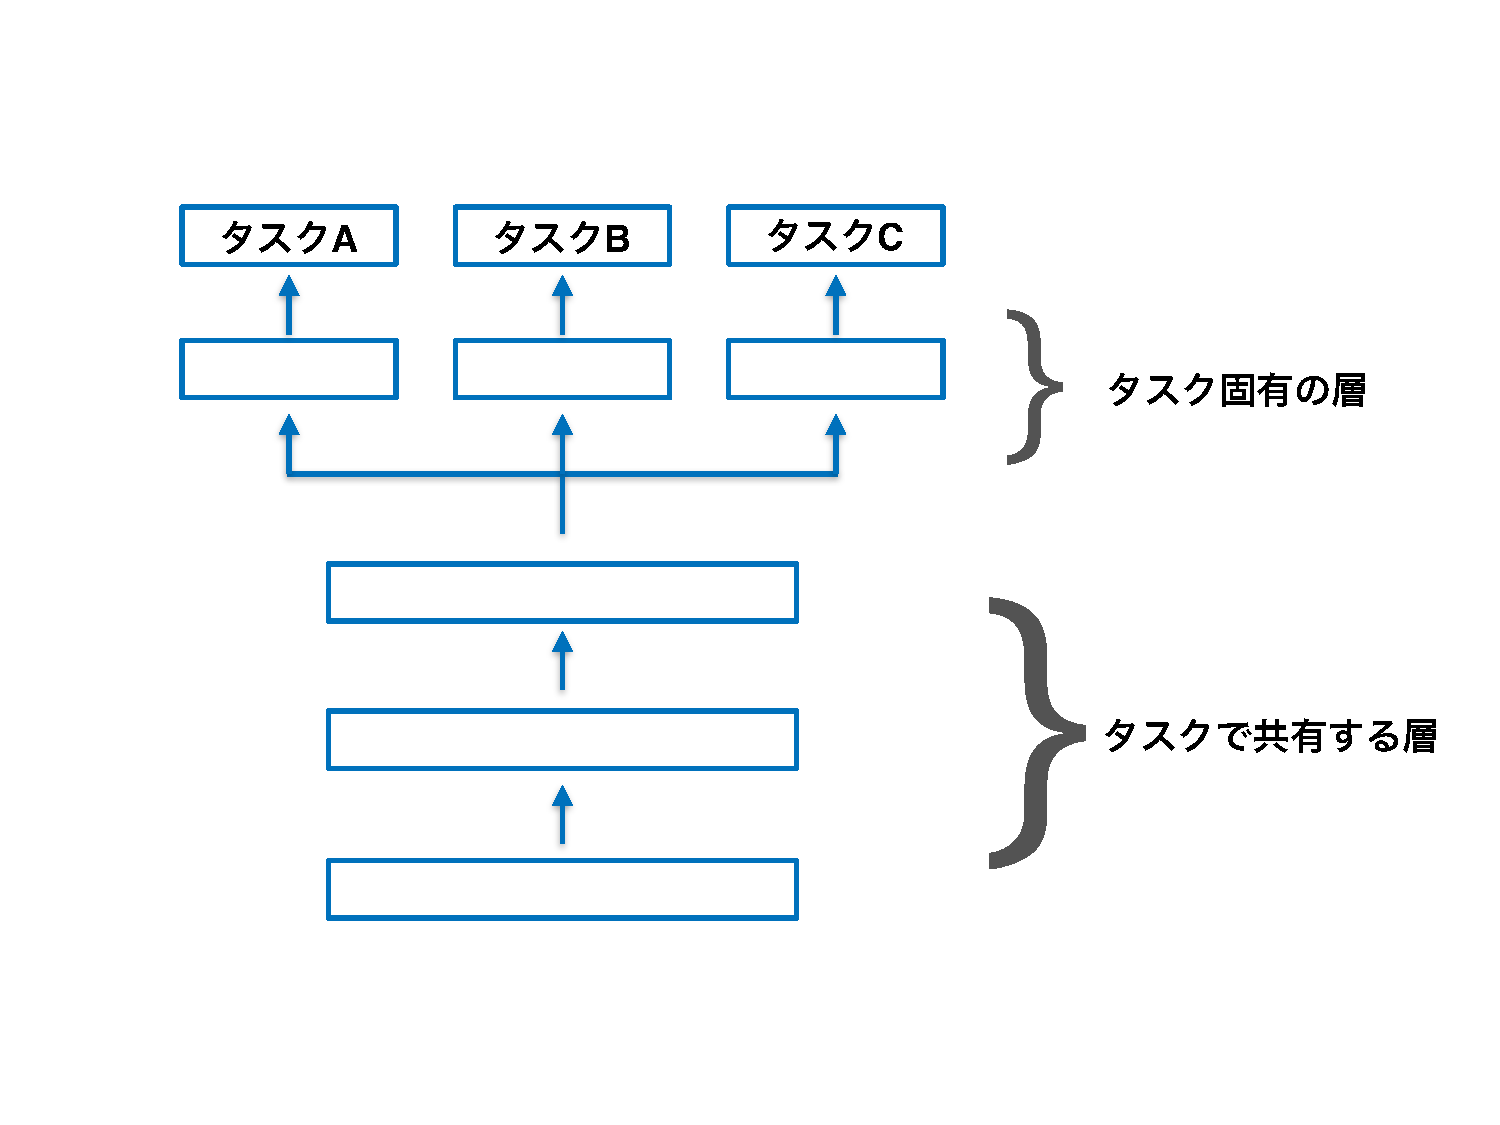
\includegraphics[width=7cm]{images/multitask_learning_example.pdf} 
	\caption{マルチタスク学習}
	\label{multitask_learning}
\end{figure}

% 3節では,入力,出力,表記などを整理する. 
\section{問題設定}
商品を$i$,レビューを予測したい商品を$i^*$,商品集合を$I$とする.ある商品$i$に対するレビュー文を$r_i$, レビュー文の集合を$R$とする.さらに商品$i$のレビューのスコアを$s_i$とする.
$i^*$のレビューを予測したいドメインを$T$とおき,$r_{i^*}$, $s_{i^*}$ともに存在するドメインを$S$とする.ここでドメインTにおけるアイテム集合を$I^T$,レビュー文を$r^T$,レビュー文集合を$R^T$ ,スコアを$s^T$と表記する.ここで$I^T \cap I^S \neq \emptyset$であり,$i^* \in I^S$, $i^* \notin I^T$であることに注意する.
また,$T$におけるユーザグループを$U^T$,$S$におけるユーザグループを$U^S$とし,$U^T \cap U^S = \emptyset $である.

$R^S_i$を入力として,$s^T_i$と$R^T_i$を正解として学習を行い,$R^S_{i^*}$から$s^T_{i^*}$を予測するモデルを提案する.

\section{提案手法}\label{suggestion}
\begin{figure}[tb]
	\centering
	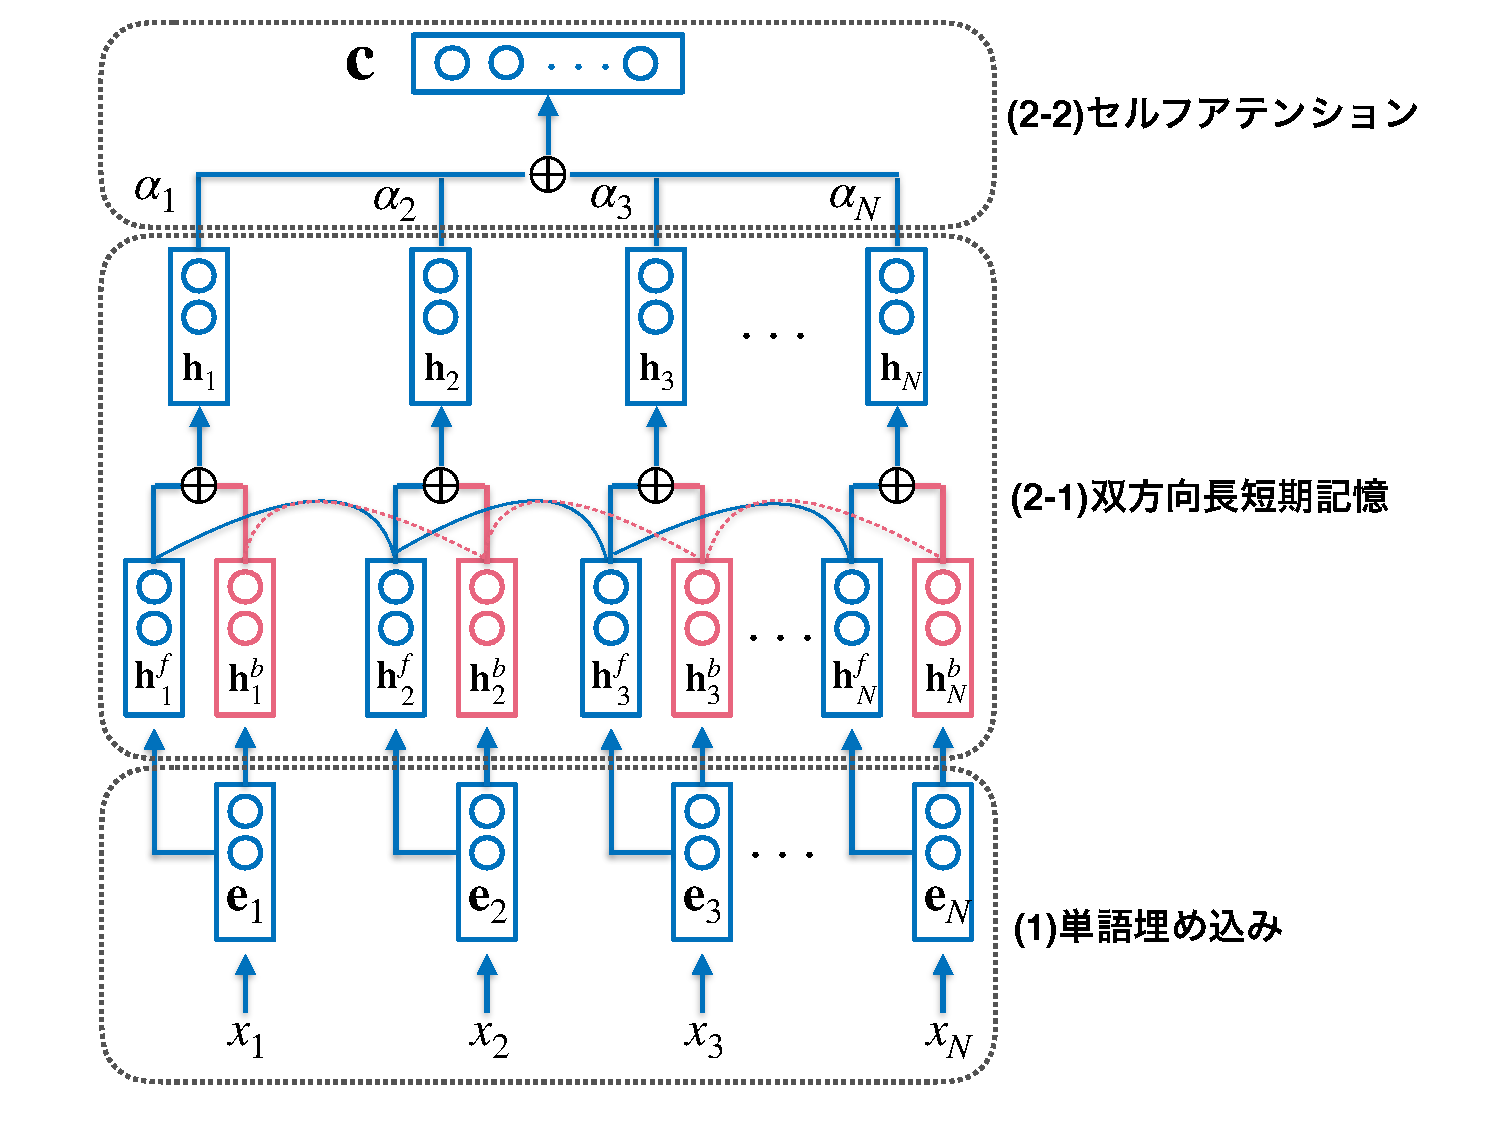
\includegraphics[width=7cm]{images/encoder2.pdf} 
	\caption{エンコーダー}
	\label{encoder}
\end{figure}
\begin{figure}[tb]
	\centering
	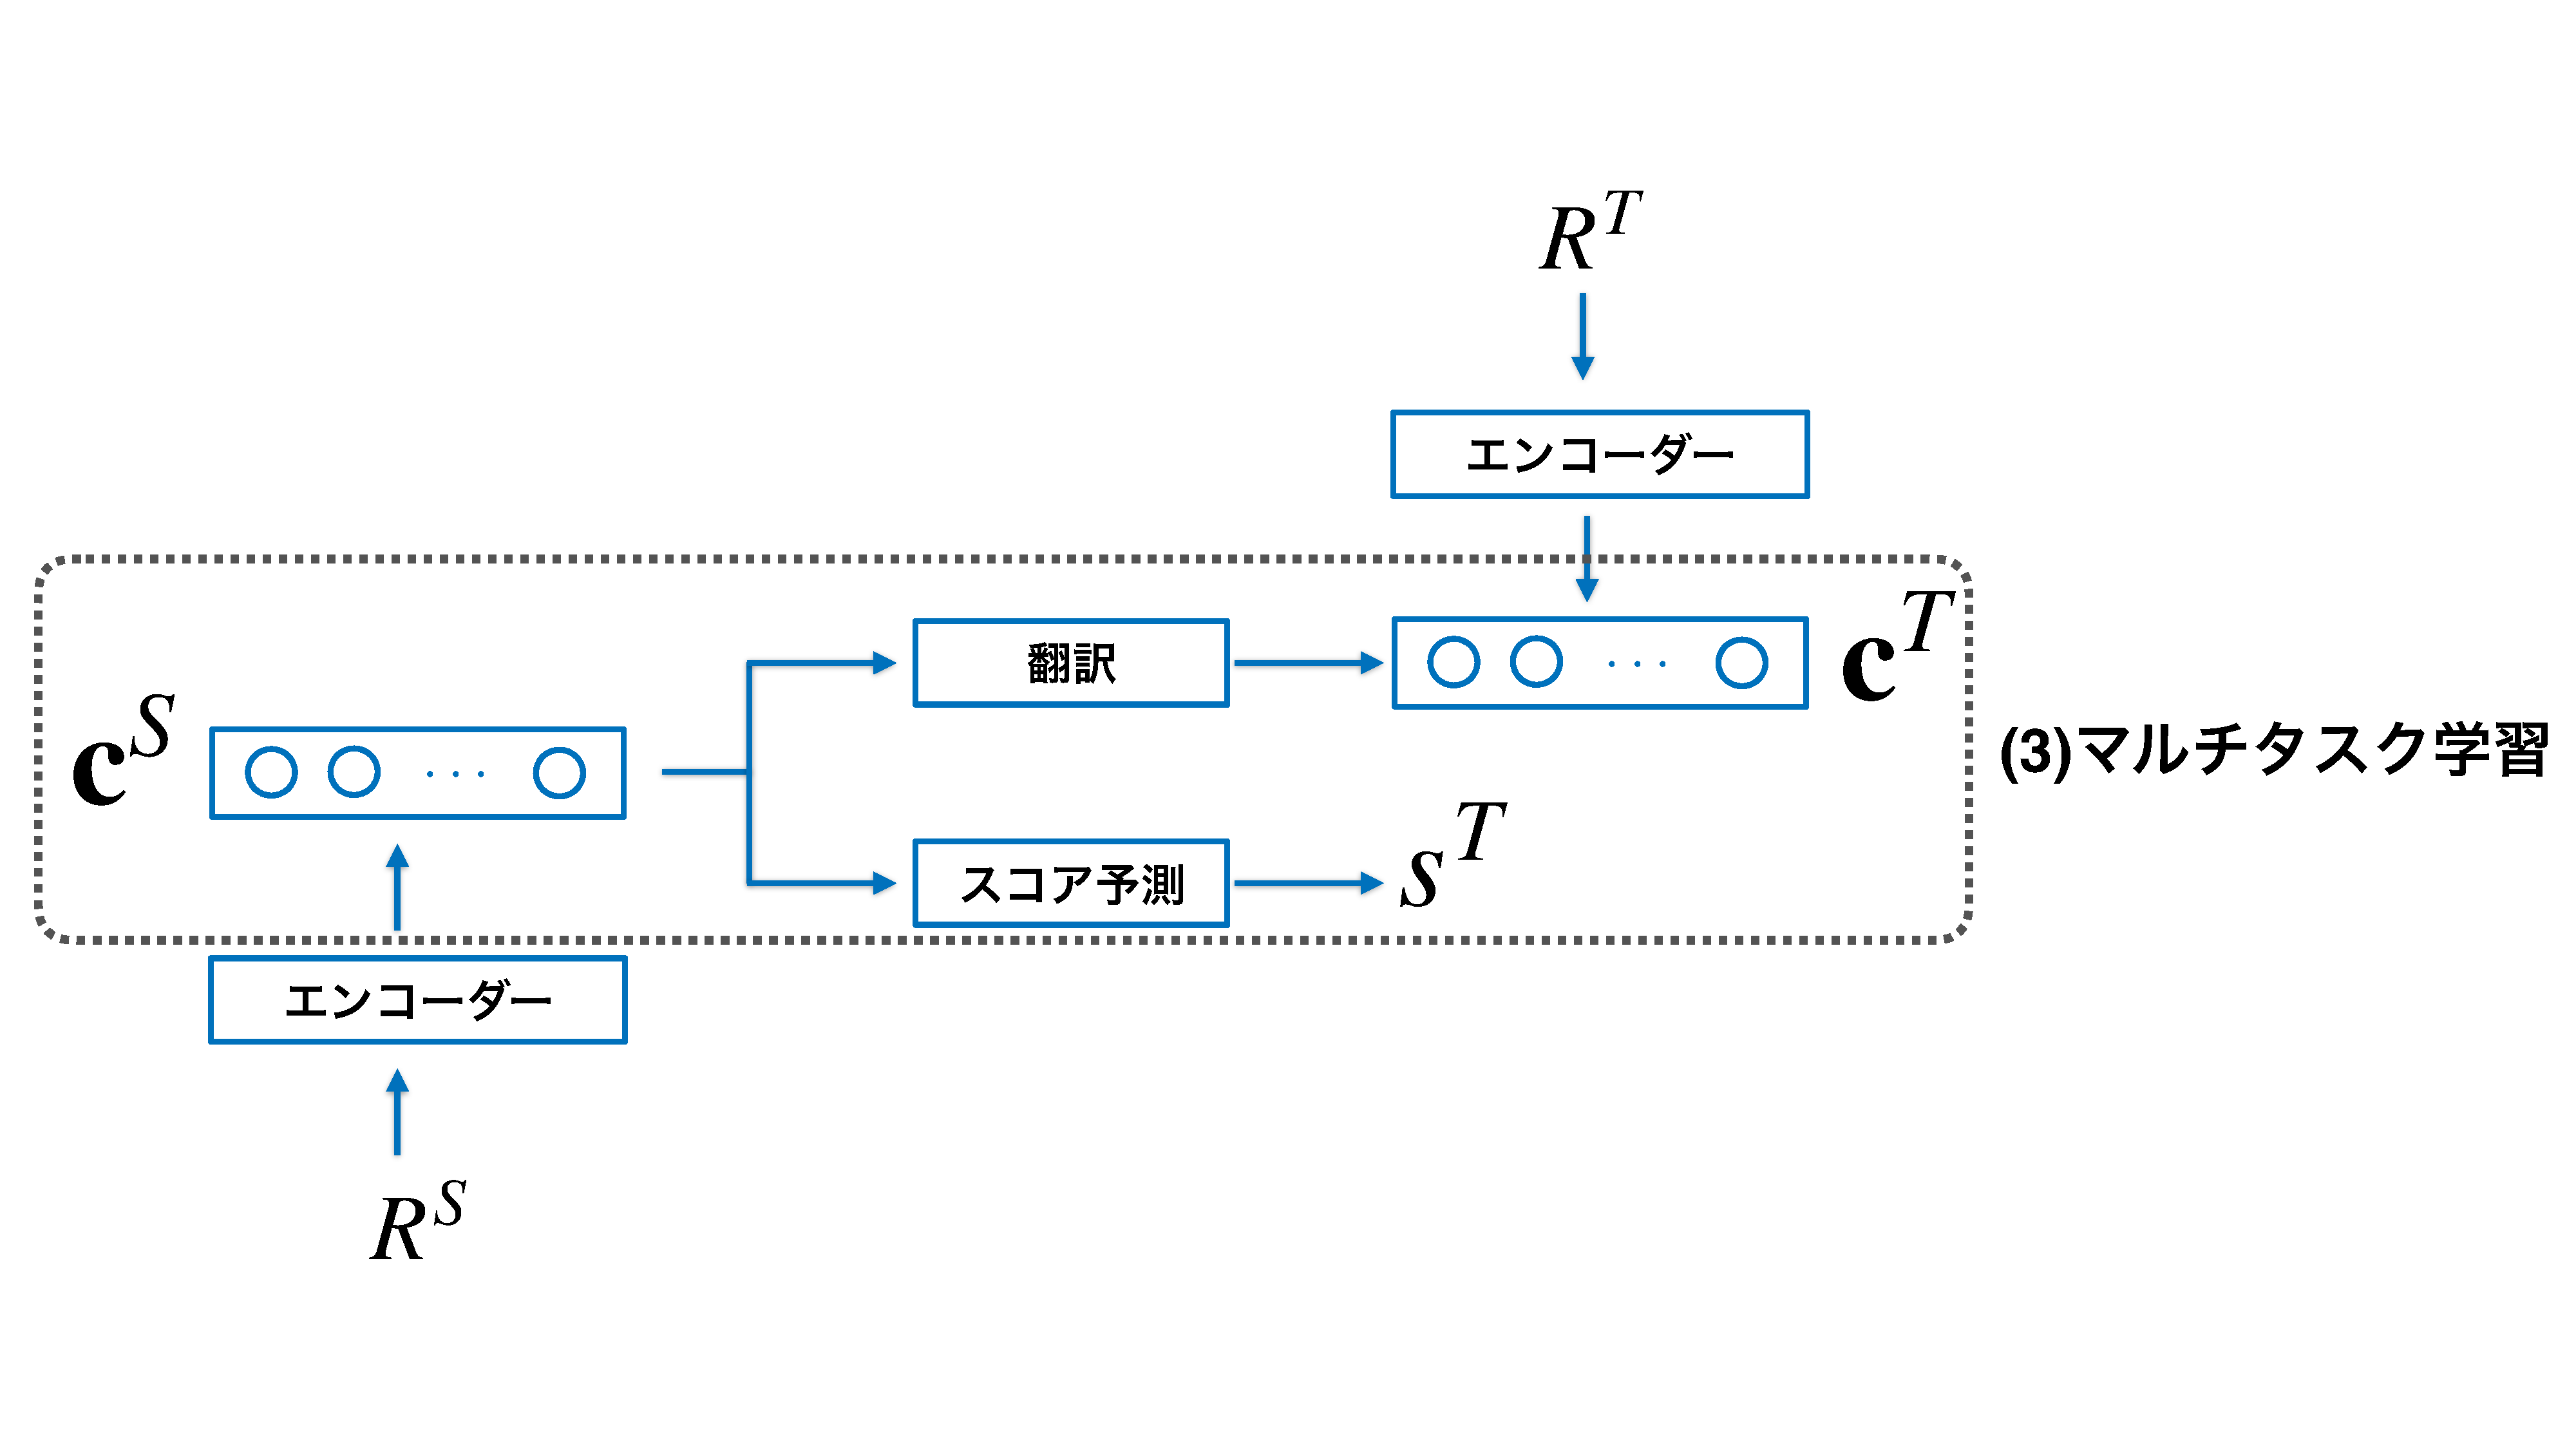
\includegraphics[width=7cm]{images/multitaskLearning.pdf} 
	\caption{マルチタスク学習}
	\label{multitaskLearning}
\end{figure}
本節では,マルチタスク学習を用いることで,まだ対象商品のレビューが存在しないドメインにおけるレビューのスコアを予測するモデルを示す.

図\ref{encoder}, \ref{multitaskLearning}に示す通り,本論文で提案するモデルは主に下記の3つのステップから構成される:

(1)$R^S_i$と$R^T_i$を入力として,単語のベクトル表現を得る.

(2)$R^S_i$と$R^T_i$の文のベクトル表現を得る.

(3)マルチタスク学習を適用して,$R^S_i$から$R^T_i$への翻訳のタスクと,$R^S_i$から$s_i^T$を予測するタスクを同時に学習する.

このモデルにおいて最も重要なアイデアは,マルチタスク学習において,$R^S_i$から$R^T_i$を予測するモデルを学習することによって,$R_i^T$を予測する上で重要な特徴量をモデルが学習し,より$s_i^T$を正確に予測できるような$R_i^S$のベクトル表現を得ることができるようになるという点である.

以下の小節では,上記で述べた各ステップの詳細について述べていく.
% 提案と提案の実現方法の具体化
% 詳細を省いて手法の説明
% いくつかの要素に分解
% 問題定義をまずする
%   - 入力,出力を数学的に定義する
%   - 出力が満たすべき性質を定義する
% ここらへんで記号を導入し始める
% 本当に妥当性の高い手法か???

% ここで,QAの手法を引用する
% 言葉で十分説明できるだけのことを書く
% でかい図faff
% 個別のアーキテクチャ
\subsection{単語のベクトル表現}\label{suggestion_create}
最初のステップは,入力となるレビュー文の各単語のそれぞれ意味を捉えた単語ベクトルへの写像である.本論文ではGlove\cite{pennington2014glove}を用いて,単語を低次元の実数値ベクトルで表現する.GloveはPenningtonらによって提案されたグローバルなMatrix Factorizationとローカルなコンテキストウィンドウを組み合わせることで,単語-単語の共起を、重み付き最小2乗で学習するモデルである.

\subsection{レビュー文のベクトル表現}\label{suggestion_create}
%ページ数が足りなければRNNの説明入れても良い
% TODO: - RNN => 再帰型ニューラルネットワークと書く
二つ目のステップとして,レビュー文のベクトル表現を得るために,本論文では双方向長短期記憶(BLSTM)とセルフアテンションを用いている.
\subsubsection{双方向長短期記憶}
長短期記憶(LSTM)はHochreiterとSchmidhuberが入力系列の長期的な依存関係の問題を解決するために提案した再帰型ニューラルネットワークの一種である.\cite{hochreiter1997long}
LSTMの構成要素は,入力,忘却,出力の3種類のゲートとメモリセルである.ここで,ステップ$t$において,入力ゲートを$\bf{i}_t$,忘却ゲートを$\bf{f}_t$,出力ゲートを$\bf{o}_t$,メモリセルを$\bf{c}_t$,隠れ状態を$\bf{h}_t$とおく.$N$個の単語を含む文$X=\{ x_1, x_2, ..., x_N \}$が与えられ,その分散表現$\{\bf{e}_1, \bf{e}_2, ..., {\bf e}_N \}$とすると,各ステップ$t$において${\bf e}_t$と前の隠れ状態${\bf h}_{t-1}$がLSTMユニットに入力される.LSTMユニットの隠れ状態${\bf h}_t$は以下のようにして得られる.

\begin{eqnarray}
{\bf i}_t&=&\sigma ({\bf W}_{\bf i} {\bf e}_t + {\bf U}_{\bf i}{\bf h}_{t-1} + {\bf V}_{\bf i}{\bf c}_{t-1}) \\
{\bf f}_t&=&\sigma ({\bf W}_{\bf f} {\bf e}_t + {\bf U}_{\bf f}{\bf h}_{t-1} + {\bf V}_{\bf f}{\bf c}_{t-1}) \\
{\bf o}_t&=& \sigma ({\bf W}_{\bf o} {\bf e}_t + {\bf U}_{\bf o}{\bf h}_{t-1} + {\bf V}_{\bf o}{\bf c}_{t}) \\
\tilde{{\bf c}}_t &=& {\rm tanh}({\bf W}_{\bf c} {\bf e}_t + {\bf U}_{\bf c}{\bf h}_{t-1}) \\
{\bf c}_t &=& {\bf f}_t \odot {\bf c}_{t-1} + {\bf i}_t \odot \tilde{{\bf c}}_t \\
{\bf h}_t &=& {\bf o}_t \odot {\rm tanh}({\bf c}_t) 
\end{eqnarray}
ここで,$\sigma$はシグモイド関数,${\rm tanh}$ははいパボリックタンジェント関数$\odot$は要素ごとの積,${\bf W}_{\bf i}, {\bf W}_{\bf f}, {\bf W}_{\bf o}, {\bf W}_{\bf c} \in \mathbb{R}^{d_h\times d_e} $,${\bf U}_{\bf i}, {\bf U}_{\bf f}, {\bf U}_{\bf o}, {\bf U}_{\bf c} \in \mathbb{R}^{d_h\times d_h} $,及び${\bf V}_{\bf i}, {\bf V}_{\bf f}, {\bf V}_{\bf o} \in \mathbb{R}^{d_h\times d_c} $ はモデルのパラメータである.$d_e, d_h, d_c$は単語ベクトルの次元,隠れ状態の次元,ならびに,メモリセルの次元である.

単方向のLSTMを用いた場合,入力系列が順方向のみで与えられるため,先頭付近の情報がLSTMユニットの後方付近の隠れ状態に反映されないという問題がある.Schusterらはこの問題を解決するために双方向再帰型ニューラルネットワークを提案した.\cite{schuster1997bidirectional}
この双方向再帰型ニューラルネットワークでは,再帰型ニューラルネットワークを一層追加することで,入力系列を順方向,逆方向の双方向で扱う.本論文では,この双方向再帰型ニューラルネットワークを採用し,その中でも双方向長短期記憶(BLSTM)を用いることとする.各ステップ$t$におけるBLSTMの隠れ状態は以下のように,順方向および逆方向それぞれの隠れ状態${\bf h}_t^f, {\bf h}_t^b$同士の要素ごとの和によって定義する.
\begin{equation}
  {\bf h}_t = {\bf h}_t^f \oplus  {\bf h}_t^b
\end{equation}
\subsubsection{セルフアテンション}
本論文ではさらに,このBLSTMの各単語に対応する隠れ層を入力として,セルフアテンションを用いる.アテンション技術は, 画像処理のタスクにおいて,画像のどの部分に着目するべきかについて取り組まれ\cite{larochelle2010learning},その後 Bahdanauらが機械翻訳におけるアテンションを提案し\cite{bahdanau2014neural},その高い精度と汎用性から自然言語処理においても注目を集めるようになった技術である.アテンションとは一般的に,入力されたデータで,どの部分に注目するべきかを決定する手段である.
入力を$\{ {\bf h}_1, {\bf h}_2, ..., {\bf h}_N \}$のベクトル集合,各入力ベクトルに対するアテンション分布を$\alpha = [\alpha_1, \alpha_2, ..., \alpha_N]$($\Sigma_n \alpha_n = 1$)とした時,以下のように,${\bf h}$の重みつき総和であるコンテキストベクトル${\bf c}$を出力する.
\begin{eqnarray}
  \alpha_j &=& \frac{{\rm exp}(S({\bf h}_j, {\bf s}))}{  \Sigma_{k=1}^N {\rm exp}(S({\bf h}_k, {\bf s}))  } \\
  {\bf c} &=& \sum_{j=1}^N \alpha_j {\bf h}_j
\end{eqnarray}
${\bf h}_j$に対するアテンションの重み$\alpha_j$は式(8)のように,ベクトル${\bf h}_j$とクエリ$\bf{s}$を引数とするスコア関数$S$に基づいて計算される.
本論文ではデータが単一の情報元から得られる文書分類タスクであるため,その中でもセルフアテンションを用いる.
通常はアテンションの対象となる情報源に対し,別の情報をクエリとして用いるが,セルフアテンションでは同一の情報源飲みを用いてアテンションを行う.セルフアテンションを行うことで,同一分中で離れた単語の関係性の理解が容易になる.
また,Linらが提案したように,クエリを用いないアテンションも一種のセルフアテンションと見なすことができ\cite{lin2017structured},本論文でもこのセルフアテンションを採用している.クエリを用いないアテンションは以下のように表される.
\begin{eqnarray}
  S({\bf x}_j) &=& {\bf v}^\mathsf{T} {\rm tanh}(W{\bf x}_j) \\
  \alpha_j &=& \frac{{\rm exp}(S({\bf x}_j))}{  \Sigma_k{\rm exp}(S({\bf x}_k))  } \\
  {\bf c} &=& \sum_j \alpha_j {\bf h}_j
\end{eqnarray}
出力のコンテキストベクトル$\bf c$はセルフアテンションの重み付で各単語に対応する隠れ層を足し合わせたものであり,レビュー文を一つのベクトルで表現したものとなる.

本論文では,商品$i$に対して,$N$個のレビューを持つドメイン$S$におけるレビュー集合$R^S_i = \{r^S_{i, 1}, r^S_{i, 2}\, ..., r^S_{i, N}\}$とM個のレビューを持つドメインTにおけるレビュー集合$R_i^T = \{ r^T_{i, 1}, r^T_{i, 2}, ..., r^T_{i, M}\}$が与えられた時,$\{r^S_{i, 1}, r^S_{i, 2}\, ..., r^S_{i, N}\}$と$\{r^T_{i, 1}, r^T_{i, 2}\, ..., r^T_{i, M}\}$をステップ2におけるエンコーダーの入力として,それぞれのコンテキストベクトル${\bf c}^S_i$と${\bf c}^T_i$を得る.ただし,${\bf c}^S_i$と${\bf c}^T_i$は以下のように計算する.
\begin{eqnarray}
 {\bf c}^S_i &=& {\bf c}^S_{i, 1} \oplus  {\bf c}^S_{i, 2} \oplus \cdots \oplus {\bf c}^S_{i, N} \\
  {\bf c}^T_i &=& {\bf c}^T_{i, 1} \oplus  {\bf c}^T_{i, 2} \oplus \cdots \oplus {\bf c}^T_{i, N}
\end{eqnarray}

\subsection{マルチタスク学習}\label{suggestion_create}
最後のステップとして,図\ref{multitaskLearning}に示す通り,マルチタスク学習によって,ステップ2で得たコンテキストベクトル${\bf c}^S$から$ {\bf c}^T$への翻訳タスクと,${\bf c}^S$から$s^T_i$を予測するタスクを同時に学習する.

Word Embedding based Correlation (WEC) Model\cite{shen2017word}はShenらがQuestion/Answer Matchingというタスクにおいて提案したモデルである.このモデルでは質問に対する答えを,ベクトル表現された質問文から,ベクトル表現された答えの文に変換する翻訳行列を学習している.本論文でもこの手法を採用し,あるドメインSで得られたレビューとあるドメインSで得られたレビューへの変換行列を学習する.すなわち翻訳行列を$M$とした時,$ M{\bf c}^S$と$ {\bf c}^T$の誤差が少なくなるように$M$のパラメータを学習する.
 
本論文におけるマルチタスク学習では,${\bf c}^S$と$ {\bf c}^T$を獲得する際のエンコーダーのパラメータを共有し,その後翻訳タスクとスコアの予測タスクでそれぞれ個別に学習する.
翻訳タスク,スコアの予測タスク共に損失関数として,平均二乗誤差を用いる.翻訳タスクにおける変換した値を$\hat{\bf c}_i$,損失関数を$L_{\rm translation} $,スコアの予測タスクにおける予測した値を$\hat{s}_i$,損失関数を$L_{\rm score}$とおき,損失関数をそれぞれ以下のように定義する.
\begin{eqnarray}
 L_{\rm translation} &=& \frac{1}{N} \sum_{i=1}^N({\bf c}_i^T - \hat{\bf c}_i) \\
 L_{\rm score} &=& \frac{1}{N} \sum_{i=1}^N({s}_i^T - \hat{s}_i)
\end{eqnarray}
ただし$N$は商品数とする.この時マルチタスク学習における目的関数$L$を以下のように定義する.
\begin{equation}
  L = \beta L_{\rm score} +  (1-\beta) L_{\rm translation}
\end{equation}
ここで$\beta$はハイパーパラメタであり,本論文における目的であるスコアの予測に対して,どの程度翻訳を考慮するかを決定する.

\section{実験}\label{experiment}
% 実験内容の具体化
% 実験の設定を詳細に記述()パラメータを含める
% 傾向: グラフ, 詳細値: 表
% グラフの説明=> グラフの読み取り方,読み取れる事柄,確かな結論,そこから推測できること
% 事実と推測は分けて書く
\subsection{データセット}\label{dataset}
実験ではAmazonが公開しているデータ\footnote{https://s3.amazonaws.com/amazon-reviews-pds/readme.html}を用いた.このデータには1995年から2015年までの,5ヵ国(アメリカ,イギリス,日本,フランス,ドイツ)におけるの商品に対するレビュー文,スコア,カテゴリ,商品IDなど15のメタデータが含まれている.本論文では,二つの国で共通に販売されている商品のレビューデータを用いるため,共通のデータが多かったアメリカとイギリスのデータを利用している.また,ある商品に対するアメリカにおけるレビュー文とイギリスにおけるレビュー文を共に学習に使うため,共に10以上レビュー文が存在する商品のみを扱う.表\ref{num_of_data}に示す通り,アメリカとイギリスに共通に存在する商品数は$29,426$件,それぞれアメリカでは$4,063,476$件,イギリスでは$1,169,246$件であった.
また,図に示す通り,イギリスのレビューのスコアの分布はアメリカのレビューのスコアの分布より多少$5.0$の割合が大きかったが,平均はアメリカが$4.4$,イギリスが$4.32$であり,標準偏差はそれぞれ$0.73$と$0.72$であり,大きく差はなかったため,レビューのスコアに前処理は加えていない.
図\ref{score_diff}はアメリカとイギリスのある商品に対するレビュースコアの差の絶対値を表したものである.スコアの差が0.4以上存在するものは全体の16.4\%であった.
% 予備実験のことを書いても良いかも?

\begin{table}[tb]
\centering
\caption{英米共通して販売されている商品データ}
\begin{tabular}{lrrr}
\hline
\multicolumn{1}{c}{} & \multicolumn{1}{c}{レビュー数} & \multicolumn{1}{c}{商品数} \\ \hline
アメリカ         & 4,063,476                          & 29,426             \\
イギリス         & 1,169,246                         & 29,426                 \\ \hline
\end{tabular}
\label{num_of_data}
\end{table}

% TODO: - epsで出力
\begin{figure}[tb]
	\centering
	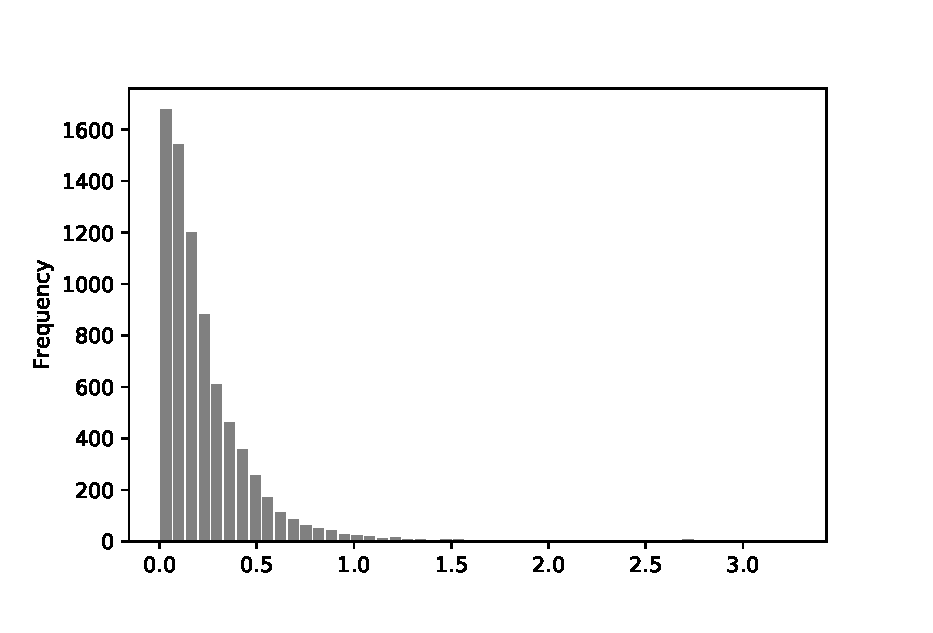
\includegraphics[width=7cm]{images/score_diff_uk_us.eps} 
	\caption{英米で販売した時の商品に対するスコアの差}
	\label{score_diff}
\end{figure}

\subsection{ハイパーパラメタと学習}\label{ex_perp}
本論文では,ニュラールネットワークは誤差逆転法で学習し,勾配法はAdam\cite{kingma2014adam}を用いた.また,単語埋め込みには,Gloveアルゴリズムを用いて英語版Wikipediaで学習済みの単語ベクトルを用いた.語彙数は$40,000$であり,$300$次元のベクトルで表現されている.
また,ハイパーパラメタはマルチタスク学習において共有しているLSTMの隠れ層には$100$,学習率には$0.001$,マルチタスク学習における$\beta$には0.5を用いた.

\subsection{レビューのスコア分類}\label{ex_create}
一つ目の実験として,ある商品におけるレビューのスコアが,イギリスにおいてアメリカよりも良くなるかか,悪くなるかの2値分類をするの実験を行った.

ベースライン手法としては,サポートベクターマシン(SVM)と通常のマルチタスク学習を用いない双方向長短期記憶(BLSTM)とセルフアテンションを用いたモデルの二つを採用した.ベースライン手法では,$R^S_i$を入力とし,$s^T_i - s^S_i \geq 0$ならば1を, $s^T_i - s^S_i < 0$ならば0を出力として学習を行った.用いたデータは提案手法同様,アメリカとイギリス共に商品のレビュー文が10以上存在するものを用いた.一方で,提案手法ではマルチタスク学習を行うため,$R^S_i$だけでなく$R^T_i$も入力し,$s^T_i - s^S_i \geq 0$ならば1を, $s^T_i - s^S_i < 0$ならば0を出力として学習を行った.

表\ref{score_classification_result}はベースライン手法と提案手法を各分類クラスのF値のマイクロ平均によって評価した結果を示す.マルチタスク学習を用いる場合,用いない場合より2.1\%の改善がみられた.LiuらのRNNによるレビュー文書の分類\cite{liu2016recurrent}においても,マルチタスク学習によって平均で2\%の精度の改善が報告されており,本論文でも同程度のマルチタスク学習による精度の改善が見られたと考えられる.

\begin{table}[tb]
\centering
\caption{レビューのスコア分類}
\begin{tabular}{lr}
\hline
\multicolumn{1}{c}{} &  \multicolumn{1}{c}{F値}\\ \hline
SVM         & 0.547         \\
BLSTM+Attention         & 0.557            \\ 
提案手法      &  \bf{0.578}            \\ \hline
\end{tabular}
\label{score_classification_result}
\end{table}


\subsection{レビューのスコアの差の予測}\label{ex_create}
二つ目の実験として,イギリスとアメリカのある商品におけるレビューのスコアの差を予測する実験を行った.

ベースライン手法としては,サポートベクター回帰(SVR)と,双方向長短期記憶(BLSTM)とセルフアテンションを用いたモデルの二つを採用した.
ベースライン手法では,$R^S_i$を入力とし,$s^T_i - s^S_i$を出力として学習を行った.用いたデータは提案手法同様,アメリカとイギリス共に商品のレビュー文が10以上存在するものを用いた.
一方で,提案手法ではマルチタスク学習を行うため,$R^S_i$だけでなく$R^T_i$も入力し,$s^T_i - s^S_i$を出力として学習を行った.

表\ref{score_diff_result}はベースライン手法と提案手法を平均二乗誤差によって評価した結果を示す.
マルチタスク学習を用いた場合,用いない場合より$0.015$の改善した.

\begin{table}[tb]
\centering
\caption{レビューのスコアの差の予測}
\begin{tabular}{lr}
\hline
\multicolumn{1}{c}{} & \multicolumn{1}{c}{平均二乗誤差} \\ \hline
SVM         & 0.267 \\
BLSTM+Attention         & 0.124       \\ 
提案手法         &  \bf{0.109}    \\ \hline
\end{tabular}
\label{score_diff_result}
\end{table}

\section{まとめ}\label{matome}

% 前半部: アブストラトの内容を 過去形にして,実験内容とその結果をやや多めにする
%本論文における貢献は,これまで研究されてこなかった越境ECにおける商品レビューに基づくスコア予測のタスクを提案し,この問題においてマルチタスク学習が有効であることを示したことである.
本研究では,越境ECのようなレビューがまだ存在しないドメイン$T$における商品のレビューのスコアを予測するタスクを提案し,また,その手法としてマルチタスク学習を用いることを提案した.我々は,マルチタスク学習によって,$R_i^S$から$s_i^T$を予測すると同時に,$R_i^S$から$R_i^T$へと翻訳するタスクを学習することで,$s_i^T$をより正確に予測するような$R_i^S$のベクトル表現を獲得することを可能とした.実験では,ドメイン$S$で売っていた商品をドメイン$T$で売った際にレビューのスコアがよくなるか,悪くなるかの2値分類タスクと,その際のレビューのスコアの差の予測タスクを行い,どちらの実験においてもマルチタスク学習を行うことで,精度が改善することを明らかにした.

また,今後の課題として以下の2点をあげる:

(1)本論文の実験ではある商品に対して各ドメインのレビュー文を10ずつ用いているが,より多くのレビューを用いることで,より正確に予測する.

(2)本論文では,ある商品に対する10のレビューのベクトル表現を足しているが,その際にもセルフアテンションを用いて,10のレビューのうち,どのレビューがより重要であるかを考慮する.
% 後半部: 今後の課題とか本論文の貢献とか


\section{謝辞}\label{Acknowledgement}
本研究に取り組むにあたって熱心にご指導してくださった加藤誠准教授に深く感謝申し上 げます.

\begin{comment}
\end{comment}


%\vspace{30mm} <- 文献が本文と近すぎるときは適宜利用してください.
\vspace{2em}


\bibliographystyle{junsrt}
\bibliography{ref}


\end{document}
